\documentclass{cornouaille}


\begin{document}


\fexo{TS}{C11 Variables à Densité}{}

\tableofcontents

\section{{Variables aléatoires à densité}{}}



\begin{exemple}
Dans une bouteille vide de contenance 1,5 litres, on verse
une quantité au hasard d'eau. On considère la variable aléatoire $X$
égale à ce volume d'eau en litres. Cette quantité peut être égale à
n'importe quel nombre de l'intervalle
$\left[0\ ;\ 1,5 \right]$.

Cela signifie que $X$ prend ses valeurs dans l'intervalle $\left[0\ ;\ 1,5 \right]$.
\end{exemple}



\begin{remarque}
Jusqu'à présent on a travaillé avec des variables aléatoires \textbf{discrètes} qui prennent un nombre fini de valeurs et leur loi est soit connue (binomiale ou Bernoulli), soit présentable sous la forme d'un tableau. Dans l'exemple précédent, la variable aléatoire prend une infinité de valeurs et toutes ces valeurs sont dans un intervalle de $\R$.
\end{remarque}




:::definition Définition: 


Si une fonction $f$ définie sur un intervalle $I$ est continue et
positive sur $I$ et si l'aire du domaine compris entre l'axe des
abscisses et la courbe de $f$ sur l'intervalle $I$ est égale à 1
(unité d'aire) alors on dit que $f$ est une \textbf{fonction
de densité}{} (ou une \textbf{densité de probabilité}{}).


:::



\begin{exemple}


\begin{minipage}{0.5\linewidth}
On considère la fonction $f$ définie sur $\left[-1\ ;\ 1 \right]$ par $f(x)=\left\{
\begin{array}{l}
x+1 \textrm{ si } x\in\left[-1\ ;\ 0 \right[ \\
-x+1 \textrm{ si } x\in\left[0\ ;\ 1 \right]
\end{array}
\right.$.
\end{minipage}

\hfill

\begin{minipage}{0.5\linewidth}



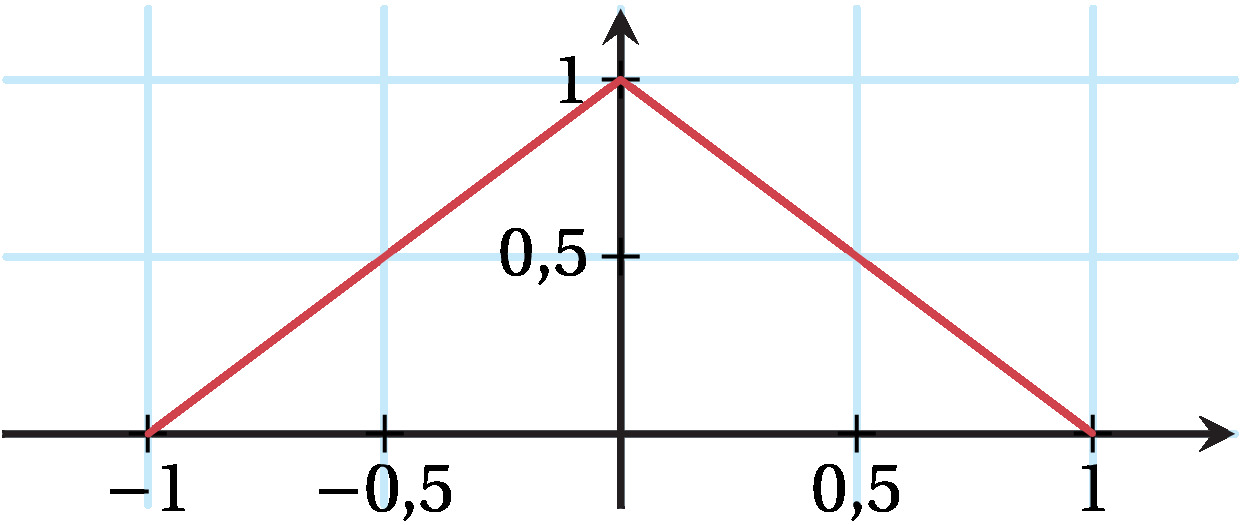
\includegraphics{./TS-Variables-0}



\end{minipage}


La fonction $f$ est positive et continue sur $\left[-1\ ;\ 1 \right]$.

De plus, le domaine entre la courbe de $f$ et l'axe des abscisses sur $\left[-1\ ;\ 1 \right]$ est un triangle d'aire $\dfrac{2\times1}{2}=1$ : la fonction $f$ est donc une fonction de densité.
\end{exemple}




:::definition Définition: 


~~


\begin{minipage}{0.65\linewidth}

Soit $f$ une fonction de densité sur un intervalle $I$.\medskip


Dire que la variable aléatoire $X$ suit la loi de densité $f$ signifie que pour tout intervalle $\left[a\ ;\ b \right]$ inclus dans $I$ on a ${P(a\leqslant X \leqslant b )=\textrm{aire}\left(\mathcal{D}\right)}$ où $\mathcal{D}$ est le domaine compris entre l'axe des abscisses, la courbe de $f$ et les droites d'équation $x=a$ et $x=b$.
\end{minipage}

\hfill

\begin{minipage}{0.3\linewidth}



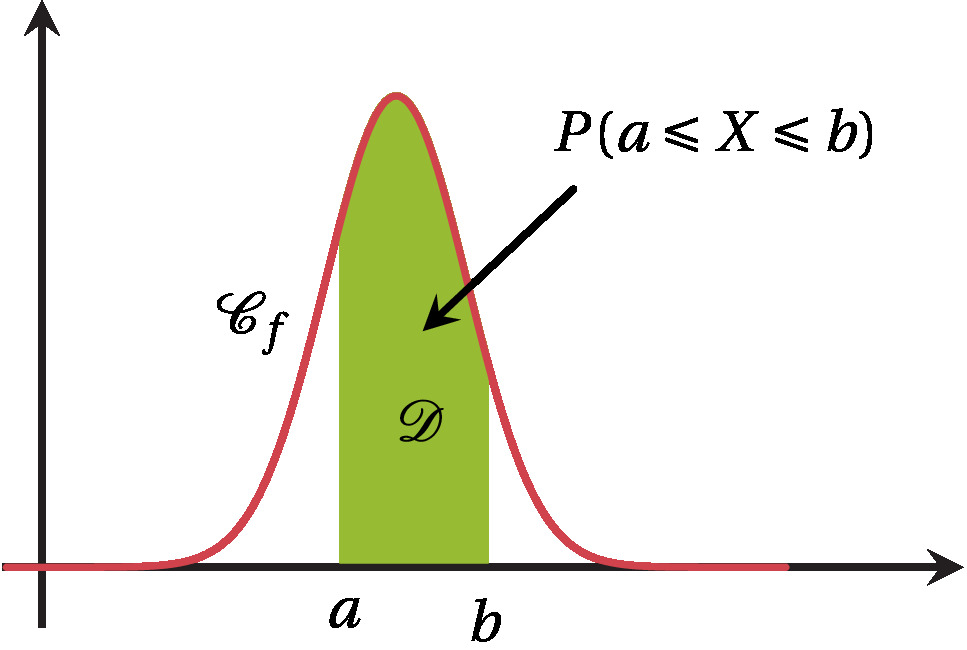
\includegraphics{./TS-Variables-1}



\end{minipage}



On a alors $P(a \leqslant X \leqslant b)=\displaystyle \int_a^b f(t) \, \textrm{d}t$.


:::



\begin{remarques}

\begin{itemize}
\item On dit alors que $X$ est une \textbf{variable aléatoire à densité}.
\item La probabilité qu'une variable aléatoire à densité $X$ prenne
une valeur $c$ est égale à 0 car $P(X=c)=\displaystyle \int_c^c f(t) \, \textrm{d}t=0$.

Par conséquent, les éventuelles inégalités strictes peuvent être remplacées par des inégalités larges dans les calculs de probabilités : par exemple $P\left(1 < X \leqslant 3\right)=P\left(1 \leqslant X \leqslant 3\right)$.

\end{itemize}

\end{remarques}



\section{Loi uniforme sur $\left[a\ ;\ b \right]$}



:::definition Définition: 



\begin{minipage}{0.6\linewidth}
Une variable aléatoire $X$ suit \textbf{la loi uniforme sur $\left[a\ ;\ b \right]$} si elle admet pour densité la fonction  constante $f$ définie sur $\left[a\ ;\ b \right]$ par $f(x)=\dfrac{1}{b-a}$.

\end{minipage}

\hfill

\begin{minipage}{0.4\linewidth}




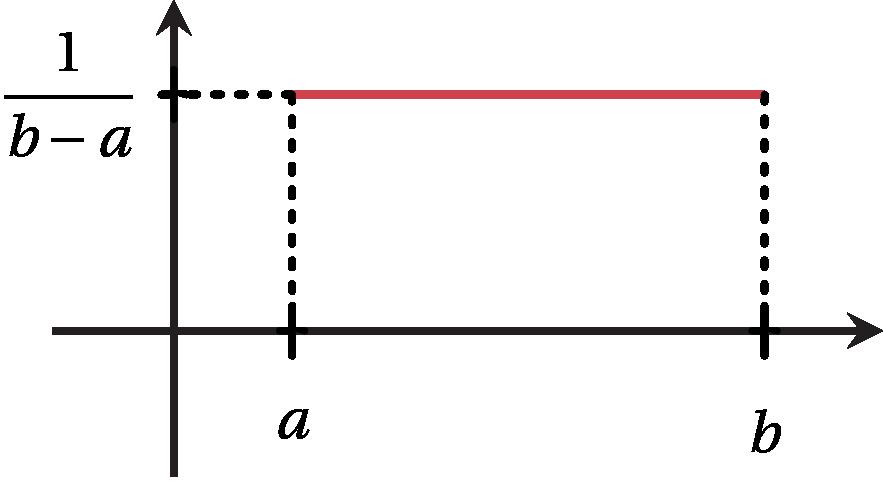
\includegraphics{./TS-Variables-2}



\end{minipage}




:::



\begin{remarque}
\og $X$ suit la loi uniforme sur $\left[a\ ;\ b \right]$ \fg{} s'écrit aussi \og $X$ suit la loi $\mathcal{U}\left(\left[a\ ;\ b \right]\right)$ \fg.
\end{remarque}



\begin{propriete}
Soit $X$ une variable aléatoire suivant la loi uniforme sur $\left[a\ ;\ b \right]$ et $\left[c\ ;\ d \right]$ un intervalle inclus dans $\left[a\ ;\ b \right]$. Alors on a $P\left(X\in\left[c\ ;\ d \right]\right)=\dfrac{d-c}{b-a}$.
\end{propriete}



\begin{preuve}
$X$ admet pour densité $f:t\mapsto \dfrac{1}{b-a}$ sur $\left[a\ ;\ b \right]$.

Donc on a $P\left(X\in\left[c\ ;\ d \right]\right)=\displaystyle \int_{c}^{d} f(t) \, \textrm{d}t=\left[\dfrac{1}{b-a}t\right]_{c}^{d}=\dfrac{d-c}{b-a}$.
\end{preuve}



\begin{propriete}
On considère une variable aléatoire $X$ suivant la loi uniforme sur $\left[a\ ;\ b \right]$ de densité $f$ et on appelle espérance mathématique de $X$ le nombre $E(X)=\displaystyle \int_{a}^{b} tf(t) \, \textrm{d}t$.

On a alors $E(X)=\dfrac{a+b}{2}$.
\end{propriete}



\begin{preuve}
On a $E(X)=\displaystyle \int_{a}^{b} tf(t) \, \textrm{d}t=\displaystyle \int_{a}^{b} \dfrac{1}{b-a} t \, \textrm{d}t=\left[\dfrac{t^2}{2(b-a)}\right]_a^b=\dfrac{b^2-a^2}{2(b-a)}$

$=\dfrac{(b-a)(b+a)}{2(b-a)}=\dfrac{a+b}{2}$.
\end{preuve}



\begin{methode}[Calculer une probabilité et une espérance pour une loi uniforme]
On utilise les différentes formules des propriétés ou on calcule à l'aide de la fonction de densité et des intégrales.

\exercice
Armand et Lise rentrent de l'école à pied. Leurs parents savent qu'ils doivent arriver entre 17h et 18h à la maison. On peut modéliser leur heure d'arrivée par une variable aléatoire $X$ suivant la loi uniforme sur $\left[17\ ;\ 18 \right]$.




\textbf{1. } Quelle est la probabilité qu'ils arrivent entre 17h et 17h15 ?


\textbf{2. } \`A quelle heure leurs parents peuvent-ils \og{}espérer\fg{} les voir arriver ?



\textbf{Correction}





\textbf{1. } Sous forme décimale, 17h15$=17,25$h puis $P(17\leqslant X \leqslant 17,25)=\dfrac{17,25-17}{18-17}=0,25$.


\textbf{2. } On a $E(X)=\dfrac{17+18}{2}=17,5$ donc leurs parents peuvent espérer les voir arriver à 17h30.






\end{methode}



\begin{remarque}
Pour la question 1 de la méthode 1, comme ${f:t\mapsto \dfrac{1}{18-17}=1}$ sur $\left[17\ ;\ 18 \right]$ est la fonction de densité de $X$, on aurait aussi pu calculer ${P(17\leqslant X \leqslant 17,25)=\displaystyle \int_{17}^{17,25} 1 \, \textrm{d}t=\left[t\right]_{17}^{17,25}=17,25-17=0,25}$.
\end{remarque}


\newpage


\section{Loi exponentielle de paramètre $\lambda$ ($\lambda>0$)}



:::definition Définition: 



\begin{minipage}{0.5\linewidth}
Une variable aléatoire $X$ suit la \textbf{loi exponentielle de paramètre}{} $\lambda$ où $\lambda>0$ si elle admet pour densité la fonction $f$ définie sur $\left[0\ ;\ +\infty \right[$ par $f(x)=\lambda\textrm{e}^{-\lambda x}$.
\vfill

~~
\end{minipage}

\hfill

\begin{minipage}{0.5\linewidth}



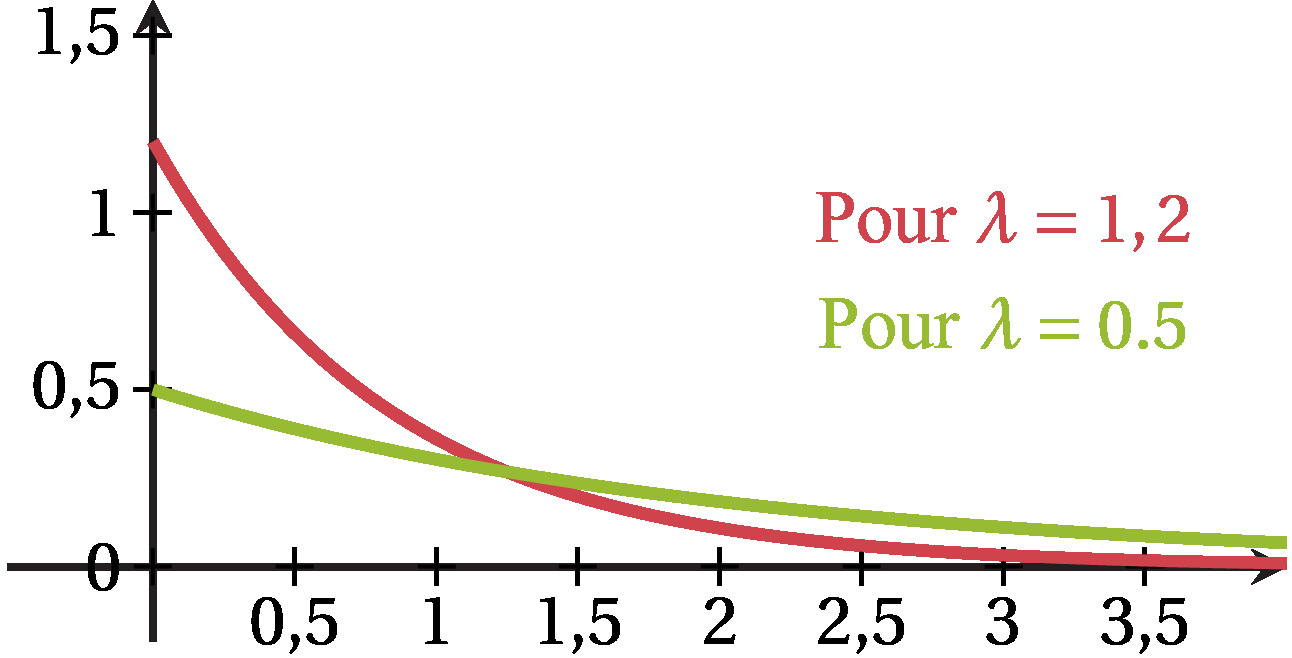
\includegraphics{./TS-Variables-3}



\end{minipage}



:::



\begin{remarque}
\og $X$ suit la loi exponentielle de paramètre $\lambda$ \fg{} s'écrit aussi \og $X$ suit la loi $\mathcal{E}\left(\lambda\right)$ \fg.
\end{remarque}



\begin{propriete}
Soit $X$ une variable aléatoire suivant la loi $\mathcal{E}\left(\lambda\right)$ et $a$, $c$ et $d$ trois réels positifs. On a alors :


\begin{minipage}{0.39\linewidth}

\begin{itemize}
\item ${P\left(c\leqslant X\leqslant d\right)=\textrm{e}^{-\lambda c}-\textrm{e}^{-\lambda d}}$
\end{itemize}

\end{minipage}

\hfill

\begin{minipage}{0.31\linewidth}

\begin{itemize}
\item $P\left(X \leqslant a \right)=1-\textrm{e}^{-\lambda a}$
\end{itemize}

\end{minipage}

\hfill

\begin{minipage}{0.25\linewidth}

\begin{itemize}
\item $P\left(X \geqslant a \right)=\textrm{e}^{-\lambda a}$
\end{itemize}

\end{minipage}






\end{propriete}



\begin{preuve}

\begin{itemize}
\item Pour tous réels $c$ et $d$ positifs, on a $P(c\leqslant X \leqslant d)=\displaystyle \int_{c}^{d} \lambda\textrm{e}^{-\lambda t} \, \textrm{d}t=\left[-\textrm{e}^{-\lambda t}\right]_{c}^{d}$ ${=-\textrm{e}^{-\lambda d}-\left(-\textrm{e}^{-\lambda c}\right)=\textrm{e}^{-\lambda c}-\textrm{e}^{-\lambda d}}$.
\item En prenant $c=0$ et $d=a$ dans le résultat précédent, on trouve $P\left(X \leqslant a \right)=P\left(0 \leqslant X \leqslant a \right)$ ${=\textrm{e}^{-\lambda \times 0}-\textrm{e}^{-\lambda a}=1-\textrm{e}^{-\lambda a}}$.
\item On a $P\left(X \geqslant a \right)=1-P\left(X<a\right)=1-P\left(X\leqslant a\right)=1-\left(1-\textrm{e}^{-\lambda a}\right)=\textrm{e}^{-\lambda a}$.
\end{itemize}

\end{preuve}




\begin{propriete}
On considère une variable aléatoire $X$ suivant la loi exponentielle de paramètre $\lambda$ de densité $f$ et on appelle espérance mathématique de $X$ le nombre $E(X)=\displaystyle \lim_{x \rightarrow +\infty} \int_{0}^{x} tf(t) \, \textrm{d}t$.

On a alors $E(X)=\dfrac{1}{\lambda}$.
\end{propriete}



\begin{preuve}
La fonction $f$ est définie sur $\left[0\ ;\ +\infty \right[$ par $f(t)=\lambda\textrm{e}^{-\lambda t}$.

Posons alors pour tout réel $t$ positif $g(t)=tf(t)=t\lambda\textrm{e}^{-\lambda t}$ : il s'agit alors de connaître une primitive de $g$ pour calculer l'intégrale.

La fonction $G$ définie sur $\left[0\ ;\ +\infty \right[$  par $G(t)=\left(-t-\dfrac{1}{\lambda}\right)\textrm{e}^{-\lambda t}$ est une primitive de $g$.

En effet $G'(t)=-1\times \textrm{e}^{-\lambda t} + \left(-t-\dfrac{1}{\lambda}\right)\times \left(-\lambda \textrm{e}^{-\lambda t}\right)=-\textrm{e}^{-\lambda t} + \lambda t \textrm{e}^{-\lambda t} + \textrm{e}^{-\lambda t} = \lambda t \textrm{e}^{-\lambda t}$.

On a alors ${\displaystyle\int_{0}^{x} tf(t) \, \textrm{d}t = \left[G(t)\right]_0^x=\left(-x-\dfrac{1}{\lambda}\right)\textrm{e}^{-\lambda x}-\left(-0-\dfrac{1}{\lambda}\right)\textrm{e}^{-\lambda 0}=-x\textrm{e}^{-\lambda x}-\dfrac{1}{\lambda}\textrm{e}^{-\lambda x}+\dfrac{1}{\lambda}}$.

On a donc $E(X) = \displaystyle \lim_{x \rightarrow +\infty} -x\textrm{e}^{-\lambda x}-\dfrac{1}{\lambda}\textrm{e}^{-\lambda x}+\dfrac{1}{\lambda}=\displaystyle \lim_{x \rightarrow +\infty} \dfrac{-\lambda x\textrm{e}^{-\lambda x}}{\lambda}-\dfrac{1}{\lambda}\textrm{e}^{-\lambda x}+\dfrac{1}{\lambda}$.

Comme $\lambda>0$, $\displaystyle \lim_{x \rightarrow +\infty} -\lambda x=-\infty$  :

\begin{itemize}
\item par composition, on a $\displaystyle \lim_{x \rightarrow +\infty} \textrm{e}^{-\lambda x}=0$.
\item par composition et croissance comparée, on a $\displaystyle \lim_{x \rightarrow +\infty} -\lambda x \textrm{e}^{-\lambda x}=0$.
\end{itemize}

Finalement, on obtient bien $E(X) = \displaystyle \lim_{x \rightarrow +\infty} \dfrac{-\lambda x\textrm{e}^{-\lambda x}}{\lambda}-\dfrac{1}{\lambda}\textrm{e}^{-\lambda x}+\dfrac{1}{\lambda}=\dfrac{1}{\lambda}$.

\end{preuve}



\begin{methode}[Calculer avec une loi exponentielle]
\exercice
On considère que le temps d'attente en minutes à un guichet du service après-vente d'un magasin peut être modélisé par une variable aléatoire $T$ suivant la loi exponentielle de paramètre 0,2.




\textbf{1. } Calculer au millième près la probabilité d'attendre un temps inférieur ou égal à 5 minutes.


\textbf{2. } Calculer au millième près la probabilité d'attendre plus de 10 minutes.


\textbf{3. } Un client se présente au guichet. Quel temps peut-il \og espérer \fg{} attendre ?



\textbf{Correction}





\textbf{1. } On calcule $P(0\leqslant T \leqslant 5)=1-\textrm{e}^{-0,2\times 5}=1-\textrm{e}^{-1}\approx 0,632$.


\textbf{2. } On calcule $P(T \geqslant 10)=\textrm{e}^{-0,2 \times 10}=\textrm{e}^{-2}\approx 0,135$.


\textbf{3. } $E(T)=\dfrac{1}{0,2}=5$ donc le client peut espérer attendre 5 minutes.




\end{methode}





\begin{remarque}
Dans le cas de la première probabilité, un calcul d'intégrale était envisageable : la fonction de densité de $T$ est la fonction définie sur $\left[0\ ;\ +\infty \right[$ par $f(t)=0,2\textrm{e}^{-0,2t}$.

La probabilité d'attendre un temps inférieur ou égal à 5 minutes est donc :

$P(0\leqslant T \leqslant 5)=\displaystyle \int_{0}^{5} 0,2\textrm{e}^{-0,2t} \, \textrm{d}t=\left[-\textrm{e}^{-0,2t}\right]_{0}^{5}=-\textrm{e}^{-0,2\times5}-\left(-\textrm{e}^{-0,2\times0}\right)=1-\textrm{e}^{-1}\approx 0,632$.
\end{remarque}



\begin{methode}[Déterminer le paramètre $\lambda$ d'une loi exponentielle]
Dans les cas où une information (probabilité ou espérance) peut être exploitée, on pose l'équation issue des formules du cours et on résout cette équation pour déterminer $\lambda$.

\exercice

Soit $X$ une variable aléatoire suivant la loi $\mathcal{E}(\lambda)$ avec $P(X\leqslant 5)=0,2$.
Déterminer $\lambda$.

\textbf{Correction}

D'après l'énoncé, on a $P(X\leqslant 5)=0,2$ donc $1-\textrm{e}^{-5 \lambda }=0,2$.

Résolvons donc cette équation : $1-\textrm{e}^{-5\lambda }=0,2 \Leftrightarrow \textrm{e}^{-5\lambda }=0,8 \Leftrightarrow \ln\left(\textrm{e}^{-5\lambda}\right)=\ln(0,8)$

$\Leftrightarrow -5\lambda=\ln(0,8)$ donc $\lambda = \dfrac{\ln(0,8)}{-5}\approx 0,045$.
\end{methode}





\begin{propriete}
Soit $X$ une variable aléatoire suivant une loi exponentielle de paramètre $\lambda>0$ et deux nombres $t>0$ et $h>0$.

La probabilité conditionnelle $P_{(X>t)}\left(X>t+h\right)$ est égale à la probabilité $P(X>h)$.

On dit que la loi exponentielle est \textbf{sans vieillissement} ou \textbf{avec absence de mémoire}.

\end{propriete}




\begin{preuve}
Par définition, on a : $P_{(X>t)}(X>t+h)=\dfrac{P((X>t)\cap (X>t+h))}{P(X>t)}$

$=\dfrac{P(X>t+h)}{P(X>t)}=\dfrac{\textrm{e}^{-\lambda(t+h)}}{\textrm{e}^{-\lambda t}}=\dfrac{\textrm{e}^{-\lambda t} \times \textrm{e}^{-\lambda h}}{\textrm{e}^{-\lambda t}}=\textrm{e}^{-\lambda h}=P(X>h)$.
\end{preuve}



\begin{exemple}
On considère un appareil dont la durée de vie en années suit la loi exponentielle de paramètre 0,05 : d'après la propriété, $P_{(X>4)}\left(X>9\right)=P_{(X>4)}\left(X>4+5\right)=P(X>5)$.

Concrètement, si l'appareil a déjà fonctionné 4 ans, la probabilité
qu'il fonctionne encore 5 ans de plus est égale à la probabilité (non
conditionnelle) qu'il fonctionne plus de 5 ans.
\end{exemple}


\section{Lois normales}



\subsection{Loi normale centrée réduite $\mathcal{N}(0\ ;\ 1)$}





:::definition Définition: 


Une variable aléatoire est centrée lorsque son espérance vaut $0$ et elle est réduite lorsque son écart-type vaut $1$.


:::



\begin{theoreme}[{\textbf{Théorème de Moivre-Laplace}{}}]
Soit $X_n$ une variable aléatoire suivant une loi binomiale
$\mathcal{B}(n\ ;\ p)$ et $Z=\cfrac{X_n-np}{\sqrt{np(1-p)}}$,
\mbox{variable} aléatoire centrée réduite.  Alors pour tous réels
$a$ et $b$ tels que $a\leqslant b$, on a :

$$
\lim_{n\rightarrow +\infty}P(a\leqslant
Z\leqslant b)=\int_a^b \dfrac{1}{\sqrt{2\pi}}
\textrm{e}^{-\dfrac{x^2}{2}} \textrm{d} x.
$$

~~


\end{theoreme}






:::definition Définition: 




\begin{minipage}{0.6\linewidth}
Une variable aléatoire $X$ suit la \textbf{loi normale
centrée \mbox{réduite}}
$\mathcal{N}(0\ ;\ 1)$ si elle admet pour densité la fonction $f$
(dont la courbe est donnée ci-contre) définie sur $\R$ par :

$$
f(x)=\dfrac{1}{\sqrt{2\pi}}\textrm{e}^{-\dfrac{x^2}{2}}.
$$
\end{minipage}

\hfill

\begin{minipage}{0.4\linewidth}



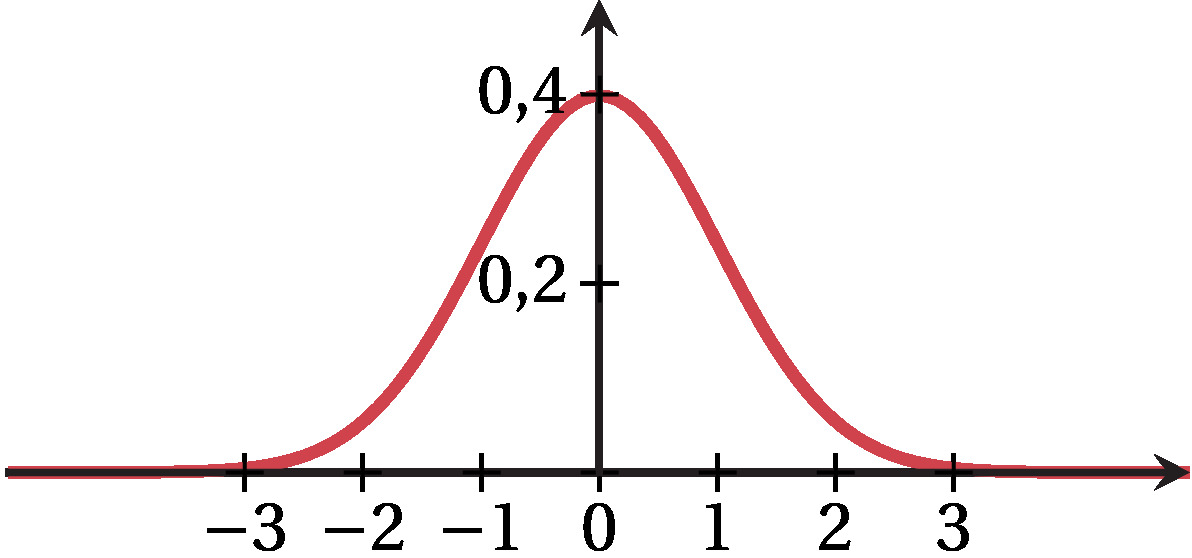
\includegraphics{./TS-Variables-4}



\end{minipage}


Autrement dit, pour tous réels $a$ et $b$ tels que $a\leqslant b$, on a :
\vspace{-0.5\baselineskip}$$P(a\leqslant X\leqslant b)=\displaystyle
\int_a^b \cfrac{1}{\sqrt{2\pi}}\text{ e}^{-\dfrac{x^2}{2}}\textrm{d} x.
$$

~~


:::





\begin{remarque}
Comme on ne peut pas calculer l'intégrale à l'aide d'une primitive
(car cette fonction de densité n'en admet pas d'explicite), on utilise
une calculatrice pour calculer des probabilités de la forme
$P(a\leqslant X\leqslant b)$ ou pour trouver un nombre $x$ tel que
$P(X\leqslant x)=p$ avec $p$ donné .
\end{remarque}




\begin{propriete}
Soit $f$ : $x\mapsto \cfrac{1}{\sqrt{2\pi}}\text{ e}^{-\dfrac{x^2}{2}}$ la fonction de densité d'une variable aléatoire suivant la loi $\mathcal{N}(0\ ;\ 1)$.

\begin{itemize}
\item L'aire totale entre \hbox{la courbe représentant la fonction de densité $f$ et l'axe des abscisses est $1$.}
\item ~~


\begin{minipage}{0.6\linewidth}
$f$ est une fonction paire, donc sa courbe représentative est symétrique par rapport à l'axe des ordonnées.

Par un argument de symétrie, pour tout réel $u$, on a :

$$
P(X\leqslant -u)=P(X\geqslant u).
$$
\end{minipage}

\hfill

\begin{minipage}{0.4\linewidth}



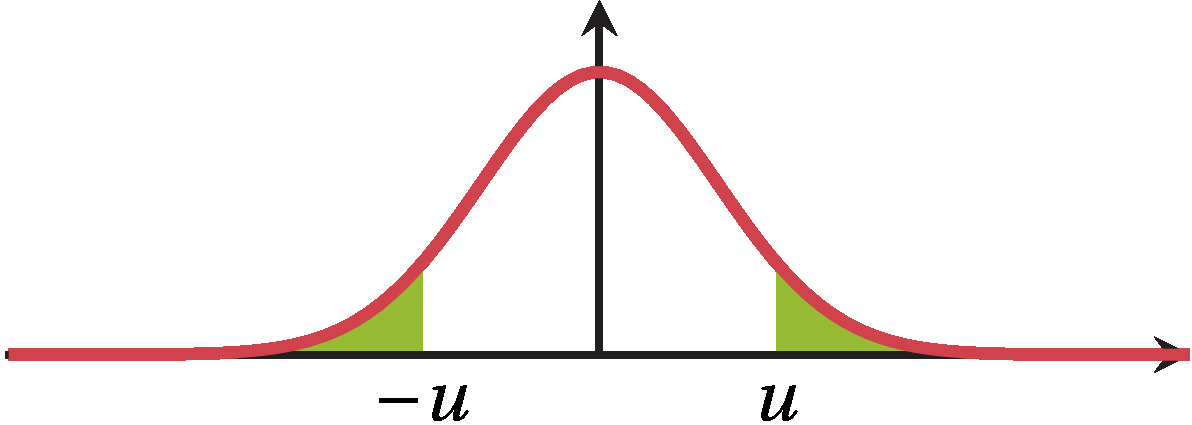
\includegraphics{./TS-Variables-5}



\end{minipage}

\end{itemize}

\end{propriete}



\begin{remarque}
Pour $u=0$, on a $P(X\leqslant 0)=P(X\geqslant 0)=0,5$.
\end{remarque}



\begin{propriete}
Soit $X$ une variable aléatoire suivant la loi normale centrée réduite $\mathcal{N}(0\ ;\ 1)$, de fonction de densité $f$. Alors

\begin{itemize}
\item $E(X)=\displaystyle \lim_{x \rightarrow -\infty}
\int_x^0 tf(t)\textrm{d} t+ \displaystyle \lim_{y
\rightarrow +\infty} \int_0^y tf(t)\textrm{d} t=0$
\qquad
\textcolor{DefSquareColor}{\rule{1.5mm}{1.5mm}}\hspace{2mm}
$V(X)=1$ et $\sigma(X)=1$.
\end{itemize}

\end{propriete}



\begin{methode}[Calculer avec la loi $\mathcal{N}(0\ ;\ 1)$]

\exercice

Soit $X$ une variable aléatoire suivant la loi normale centrée réduite $\mathcal{N}(0\ ;\ 1)$.




\textbf{1. } \`A l'aide d'une calculatrice, déterminer une valeur approchée au millième de :




\textbf{1.a) } $P(2\leqslant X\leqslant 3)$


\textbf{1.b) } $P(X\leqslant 0,7)$


\textbf{1.c) } $P(X>-0,2)$




\textbf{2. }




\textbf{2.a) } Déterminer $t$ tel que $P(X\leqslant t)=0,25$.


\textbf{2.b) } Déterminer $u$ tel que $P(X>u)=0,4$.





\textbf{Correction}




\textbf{1. } 



\textbf{1.a) } 

\textcolor{H1}{\bfseries Calculatrice TI}

\begin{itemize}
\item On accède au menu \textbf{distrib} en appuyant sur la touche \textbf{2nd}
puis la touche \textbf{VAR}
\item On choisit \verb"NormalFrep(" et on écrit \verb"NormalFrep(2,3,0,1)".
\end{itemize}
\columnbreak


\textcolor{H1}{\bfseries Calculatrice Casio}

\begin{itemize}
\item Dans le menu \textbf{RUN}, on appuie sur \textbf{OPTN}
puis \textbf{STAT} puis \textbf{DIST} puis \textbf{NORM} puis \textbf{Ncd}.
\item On écrit alors \verb"NormCD(2,3,1,0)".
\end{itemize}



On obtient  $P(2\leqslant X\leqslant 3)\approx0,021$.


\textbf{1.b) } ~~


\begin{minipage}{0.6\linewidth}
La calculatrice donne $P(0\leqslant X\leqslant 0,7)\approx 0,258$ donc

$P(X\leqslant 0,7)=P(X<0)+P(0\leqslant X\leqslant 0,7)$

$\approx 0,5+0,258=0,758$.
\end{minipage}

\hfill

\begin{minipage}{0.4\linewidth}



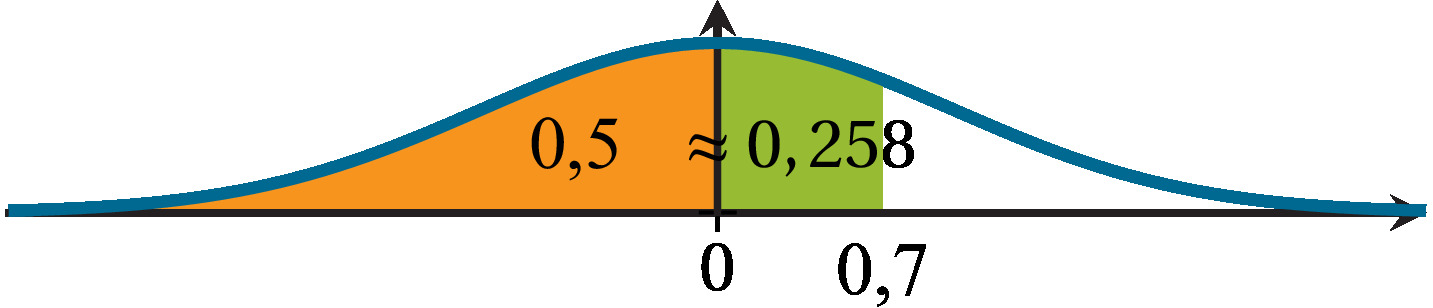
\includegraphics{./TS-Variables-6}



\end{minipage}




\textbf{1.c) } ~~





\begin{minipage}{0.6\linewidth}
La calculatrice donne $P(-0,2<X<0)\approx 0,079$ donc
$P(X>-0,2)=P(-0,2<X<0)+P(X\geqslant 0)$

$\approx 0,079+0,5=0,579$.
\end{minipage}

\hfill

\begin{minipage}{0.4\linewidth}



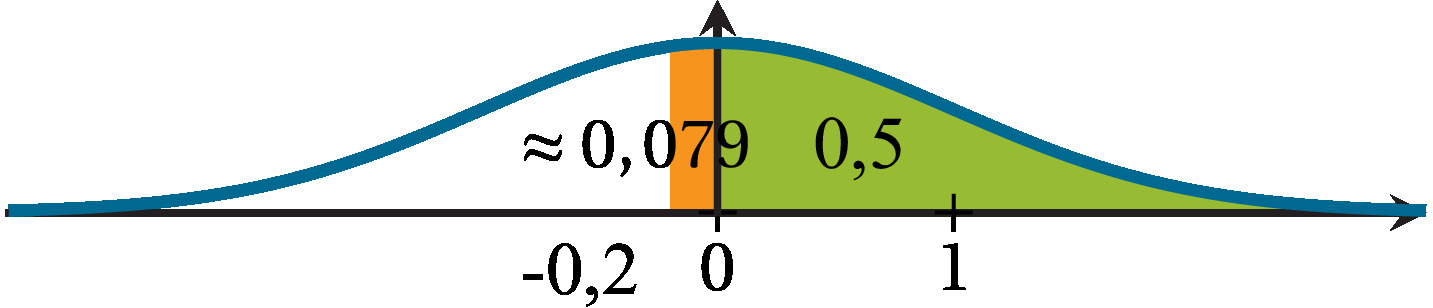
\includegraphics{./TS-Variables-7}



\end{minipage}






\textbf{2. }




\textbf{2.a) } 

\textcolor{H1}{\bfseries Calculatrice TI}

\begin{itemize}
\item \raggedright
Dans le menu
\textbf{distrib}, 


on choisit \verb"FracNormale(" et on écrit \verb"FracNormale(0.25,0,1)".
\end{itemize}


\columnbreak

\textcolor{H1}{\bfseries Calculatrice Casio}

\begin{itemize}
\item \raggedright Dans le menu 



\textbf{STAT} > \textbf{DIST} > \textbf{NORM}, on choisit
\textbf{InvN} et on écrit \verb"InvNormCD(0.25,1,0)".
\end{itemize}



On obtient $t\approx -0,674$.


\textbf{2.b) } ~~


\begin{minipage}{0.6\linewidth}
$P(X>u)=0,4 \Leftrightarrow P(X\leqslant u)=0,6$.

On trouve $u\approx 0,253$.
\end{minipage}

\hfill

\begin{minipage}{0.4\linewidth}




\includegraphics{./TS-Variables-8}



\end{minipage}






~~



~~
\end{methode}




\begin{theoreme}
Soit $X$ une variable aléatoire suivant la loi normale centrée réduite $\mathcal{N}(0\ ;\ 1)$ et $\alpha\in ]0\ ;\ 1[$. Alors il existe un unique réel $u_{\alpha}>0$ tel que $P(-u_{\alpha}\leqslant X\leqslant u_{\alpha})=1-\alpha$.
\end{theoreme}



\begin{preuve}
Soit $\alpha\in]0\ ;\ 1[$, on a alors $1-\alpha\in]0\ ;\ 1[$.



Sur $[0\ ;\ +\infty[$, soit $f:x\mapsto P(-x\leqslant X\leqslant x)=2P(0\leqslant X\leqslant x)=2\displaystyle\int_{0}^{x}\dfrac{1}{\sqrt{2\pi}}\textrm{e}^{-\cfrac{t^2}{2}}\textrm{d}t$


par symétrie de la fonction de densité de la loi $\mathcal{N}(0\ ;\ 1)$.



Comme $g:x\mapsto \displaystyle\int_{0}^{x}\dfrac{1}{\sqrt{2\pi}}\textrm{e}^{-\cfrac{t^2}{2}}\textrm{d} t$ est une primitive de $t\mapsto \dfrac{1}{\sqrt{2\pi}}\textrm{e}^{-\cfrac{t^2}{2}}$ : 
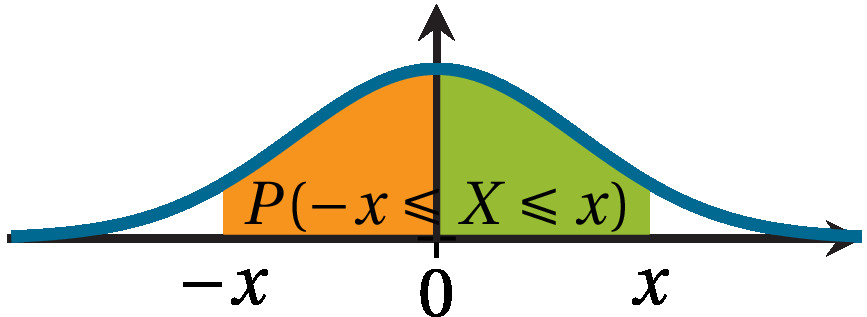
\includegraphics{./TS-Variables-9}



\begin{itemize}
\item $f=2g$ est dérivable donc \textbf{continue} sur $[0\ ;\ +\infty[$ ;


\item $f'(x)=2g'(x)=\dfrac{2}{\sqrt{2\pi}}\textrm{e}^{-\cfrac{x^2}{2}}>0$ donc $f$ est \textbf{strictement croissante} sur $[0\ ;\ +\infty[$.
\end{itemize}


De plus, $f(0)=P(-0\leqslant X\leqslant 0)=P(X=0)=0$,
${\displaystyle\lim_{x\rightarrow +\infty} f(x)=\lim_{x\rightarrow
+\infty} P(-x\leqslant X\leqslant x)=1}$
par définition d'une loi à densité. Comme
$\mathbf{1-}\alpha\mathbf{\in[0\ ;\ 1[}$, d'après le théorème de
bijection, l'équation $f(x)=1-\alpha$ admet une unique solution notée
$u_{\alpha}$ sur $[0\ ;\ +\infty[$ c'est-à-dire qu'il existe un unique
réel $u_{\alpha}> 0$ tel que
$P(-u_{\alpha}\leqslant X\leqslant u_{\alpha})=1-\alpha$.
\end{preuve}



\begin{valeurspart}En particulier, $u_{0,05} \approx 1,96$ et $u_{0,01}\approx 2,58$.

Autrement dit, $P(-1,96\leqslant X\leqslant 1,96)\approx 0,95$ et $P(-2,58\leqslant X\leqslant 2,58)\approx 0,99$.
\end{valeurspart}



\subsection{Lois normales $\mathcal{N}(\mu\ ;\ \sigma^2)$}



:::definition Définition: 

 Soit $\mu$ et $\sigma$ deux
réels avec $\sigma>0$. On dit qu'une variable aléatoire $X$ suit la
\textbf{loi normale $\mathcal{N}(\mu\ ;\ \sigma^2)$} si
$Z=\cfrac{X-\mu}{\sigma}$ suit la loi normale centrée réduite
$\mathcal{N}(0\ ;\ 1)$.


:::



\begin{remarques}

\begin{itemize}
\item Il en résulte que si $X$ suit la loi $\mathcal{N}(0\ ;\ 1)$ alors $\mu+\sigma X$ suit la loi $\mathcal{N}(\mu\ ;\ \sigma^2)$.
\item Si $X$ suit la loi $\mathcal{N}(\mu\ ;\ \sigma^2)$,
alors sa densité $f$ est donnée par
${f(x)=\cfrac{1}{\sigma\sqrt{2\pi}}\textrm{ e}^{-\cfrac{(x-\mu)^2}{2\sigma^2}}}$.


La courbe de $f$ est appelée \textbf{gaussienne} et est symétrique par rapport à la droite d'équation $x=\mu$ ce qui permet d'en déduire des probabilités par symétrie autour de $\mu$.






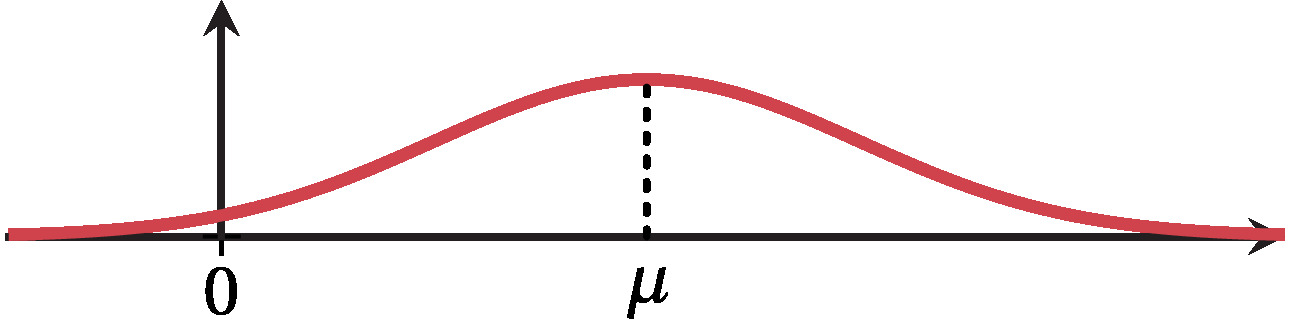
\includegraphics{./TS-Variables-10}





\end{itemize}


\end{remarques}




\begin{methode}[Calculer avec une loi $\mathcal{N}(\mu\ ;\ \sigma^2)$]

\exercice\label{methode5SP2}




\textbf{1. } Soit $X$ une variable aléatoire suivant la loi $\mathcal{N}(7\ ;\ 2^2)$.


\`A l'aide d'une calculatrice, déterminer une valeur approchée au millième de :




\textbf{1.a) } $P(6\leqslant X\leqslant 9)$


\textbf{1.b) } $P(X<10)$


\textbf{1.c) } $P(X\geqslant 8)$




\textbf{2. } Soit $Y$ une variable aléatoire suivant la loi $\mathcal{N}(6\ ;\ 3^2)$.


\`A l'aide d'une calculatrice, déterminer une valeur approchée au millième de :




\textbf{2.a) } $t$ tel que $P(Y<t)=0,95$.


\textbf{2.b) } $u$ tel que $P(Y\geqslant u)=0,1$.




\textbf{Correction}




\textbf{1. }




\textbf{1.a) } On entre \verb"NormalFrep(6,9,7,2)" ou \verb"NormCD(6,9,2,7)"
selon le modèle de calculatrice et on obtient $P(6\leqslant X\leqslant 9)\approx 0,533$.


\textbf{1.b) } ~~


\begin{minipage}{0.6\linewidth}

\begin{itemize}
\item Une calculatrice donne $P(7<X<10)\approx 0,433$ donc $P(X<10)=P(X\leqslant 7)+P(7<X<10)$

$\approx 0,5+0,433=0,933$.
\end{itemize}

\end{minipage}

\hfill

\begin{minipage}{0.4\linewidth}



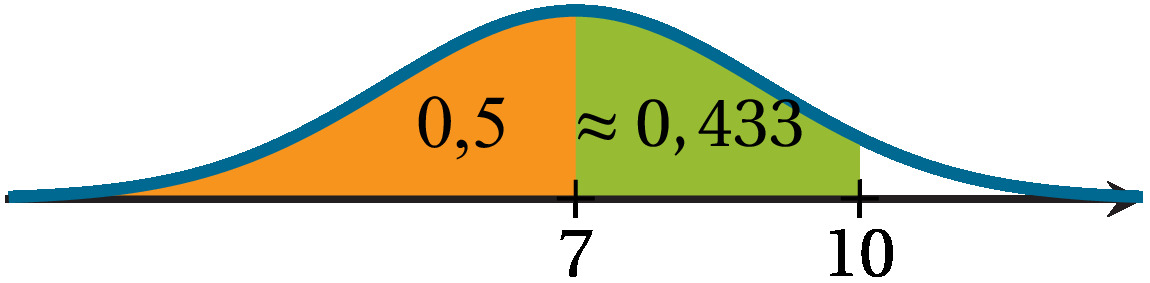
\includegraphics{./TS-Variables-11}



\end{minipage}


\begin{itemize}\smallskip
\item Pour calculer $P(X<a)$, on peut aussi calculer $P\left(-10^{99}\leqslant X<a \right)$ avec une calculatrice. On obtient alors $P\left(-10^{99}\leqslant X< 10 \right)\approx0,933.$
\end{itemize}



\textbf{1.c) } ~~





\begin{minipage}{0.6\linewidth}

\begin{itemize}
\item La calculatrice donne $P(7\leqslant X<8)\approx 0,191$ donc
$P(X\geqslant 8)=P(X\geqslant 7)-P(7\leqslant X < 8)$

$\approx 0,5-0,191=0,309$.
\end{itemize}

\end{minipage}

\hfill

\begin{minipage}{0.4\linewidth}



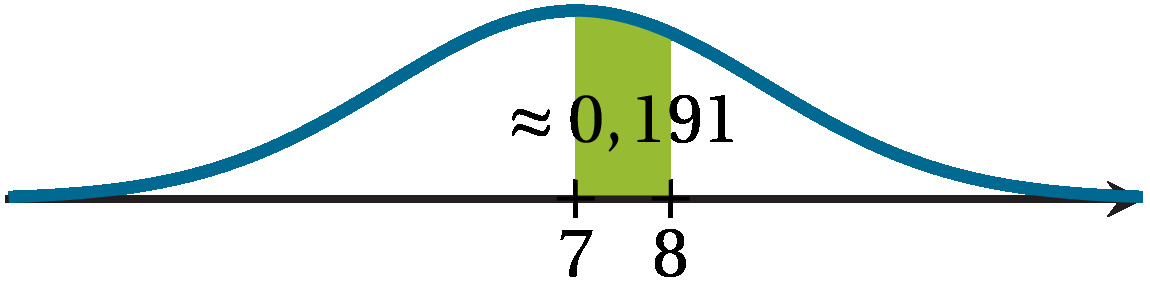
\includegraphics{./TS-Variables-12}



\end{minipage}


\begin{itemize}\smallskip
\item Pour calculer $P(X\geqslant a)$, on peut aussi calculer
$P\left(a\leqslant X\leqslant 10^{99}\right)$ avec une calculatrice. on obtient alors $P\left(8\leqslant X\leqslant 10^{99} \right)\approx0,309.$
\end{itemize}





\textbf{2. }




\textbf{2.a) } On entre \verb"FracNormale(0.95,6,3)" ou
\verb"InvNormCD(0.95,3,6)" selon le modèle de calculatrice et on obtient $t\approx 10,935$.



\textbf{2.b) }~~


\begin{minipage}{0.6\linewidth}
On a $P(X\geqslant u)=0,1 \Leftrightarrow P(X<u)=0,9$.

Une calculatrice donne $u\approx 9,845$.
\end{minipage}

\hfill

\begin{minipage}{0.4\linewidth}



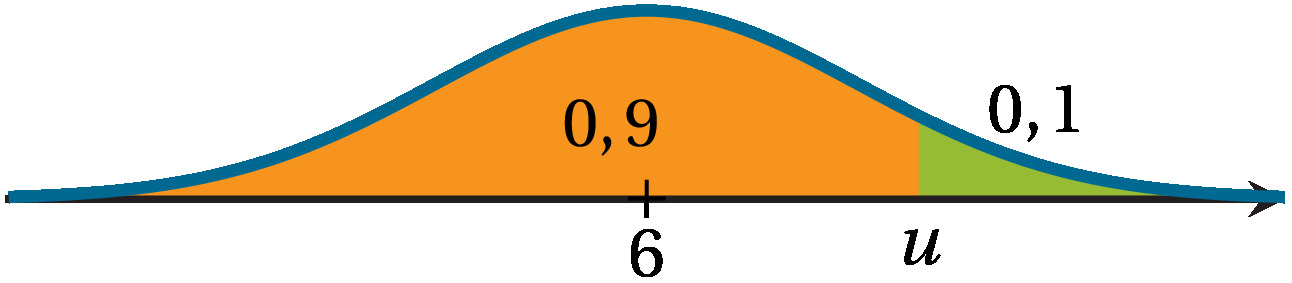
\includegraphics{./TS-Variables-13}



\end{minipage}










~~

\end{methode}



\begin{remarque} Ces méthodes utilisant le fait que $P(X\leqslant a)\approx P(-10^{99}\leqslant X\leqslant a)$ et\linebreak $P(X\geqslant a)\approx P(a\leqslant X\leqslant 10^{99})$  peuvent également être utilisées dans le cas particulier de la loi normale centrée réduite $\mathcal{N}(0\ ;\ 1)$.
\end{remarque}







\begin{propriete}
Soit $X$ une variable aléatoire suivant la loi normale $\mathcal{N}(\mu\ ;\ \sigma^2)$. On a alors :

\begin{colitemize}{2}
\item $E(X)=\mu$ ;
\item $V(X)=\sigma^2$ et $\sigma(X)=\sigma$.
\end{colitemize}


\end{propriete}



\begin{remarques}

\begin{itemize}
\item Plus $\sigma$ est petit, plus les valeurs prises par $X$ sont concentrées autour de la moyenne.




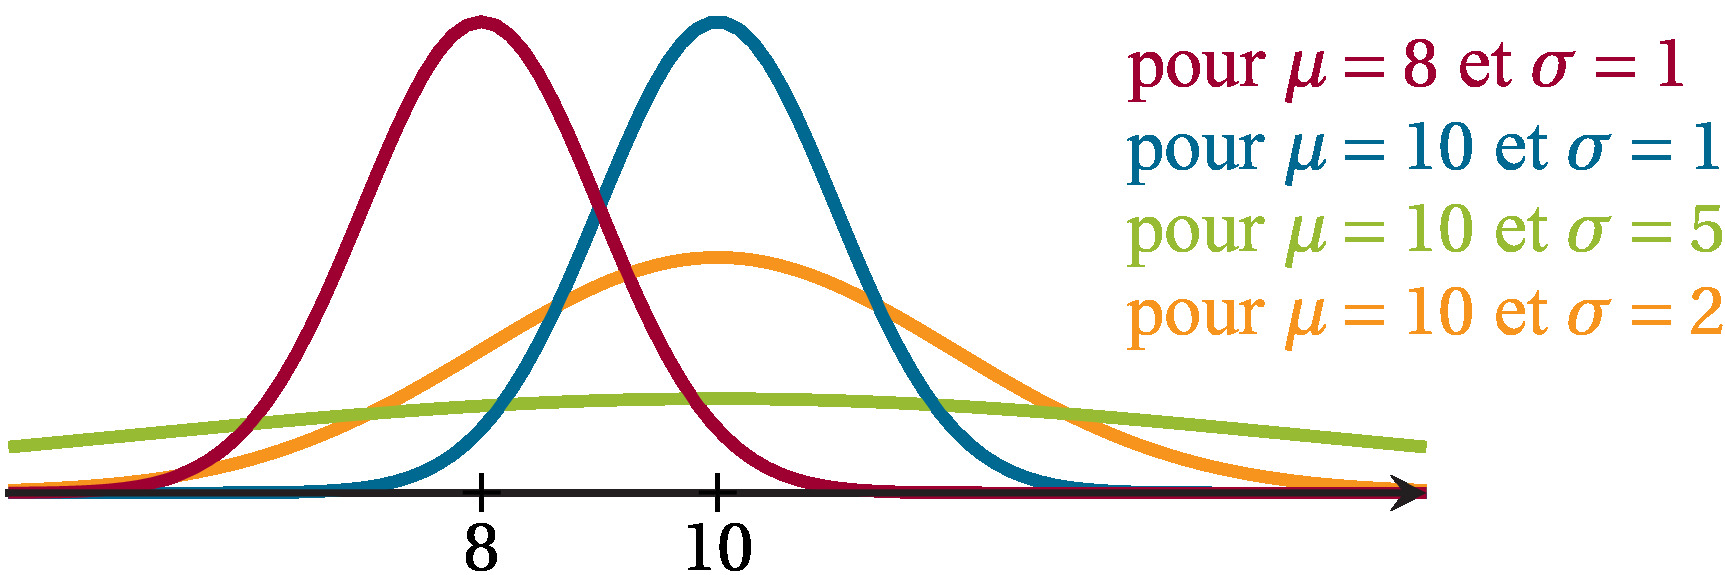
\includegraphics{./TS-Variables-14}



\item On peut considérer que sous certaines conditions (par exemple ${n\geqslant30}$, ${np\geqslant 5}$ et ${n(1-p)\geqslant5}$), la loi $\mathcal{N}(np\ ;\ \sqrt{np(1-p)}^2)$ approxime convenablement la loi $\mathcal{B}(n\ ;\ p)$.
\end{itemize}


\end{remarques}



\begin{methode}[Centrer et réduire pour déterminer des paramètres d'une loi]
Centrer et réduire une variable aléatoire suivant une loi normale de paramètre(s) inconnu(s) permet de travailler avec la loi connue $\mathcal{N}(0\ ;\ 1)$.

\exercice\label{methode6SP2} On modélise par une loi normale
d'espérance $\mu$ et d'écart-type $\sigma$ le temps $T$ (en secondes)
mis par un sportif amateur pour parcourir un 100 mètres.

Ce sportif a remarqué qu'il mettait en moyenne $13$ secondes à
parcourir la distance, et qu'il arrivait à descendre en dessous des
$12$ secondes pour $5\%$ des courses.

Déterminer les valeurs de $\mu$ et $\sigma$.

\textbf{Correction}


\begin{itemize}
\item Le temps moyen pour parcourir 100 mètres est de $13$ secondes donc l'espérance $\mu$ vaut $13$.
\item On sait de plus que $P(T\leqslant 12 )=0,05$.

Posons $Z=\dfrac{T-13}{\sigma}$, la variable aléatoire $Z$ suit alors la loi normale centrée réduite.

De plus, $T\leqslant 12 \Leftrightarrow \dfrac{T-13}{\sigma}\leqslant  \dfrac{-1}{\sigma}$ d'où $P(T\leqslant 12 )=P\left(Z\leqslant \dfrac{-1}{\sigma}\right)=0,05$.

Or, à l'aide d'une calculatrice, on trouve que le réel $u$ tel que $P(Z\leqslant u)=0,05$ vaut approximativement $-1,645$ donc $\dfrac{-1}{\sigma}\approx-1,645$ et $\sigma\approx\cfrac{1}{1,645}\approx0,608$.
\end{itemize}




~~
\end{methode}





\begin{propriete}[Quelques intervalles remarquables]
Soit $X$ une variable aléatoire suivant la loi normale $\mathcal{N}(\mu\ ;\ \sigma^2)$. On a alors  :

\begin{itemize}
\item $P(X\in[\mu-\sigma\ ;\ \mu+\sigma])=P(\mu-\sigma\leqslant X\leqslant \mu+\sigma)\approx0,68$ ;
\item $P(X\in[\mu-2\sigma\ ;\ \mu+2\sigma])=P(\mu-2\sigma\leqslant X\leqslant \mu+2\sigma)\approx0,954$ ;
\item $P(X\in[\mu-3\sigma\ ;\ \mu+3\sigma])=P(\mu-3\sigma\leqslant X\leqslant \mu+3\sigma)\approx0,997$.
\end{itemize}


Graphiquement, on a alors :




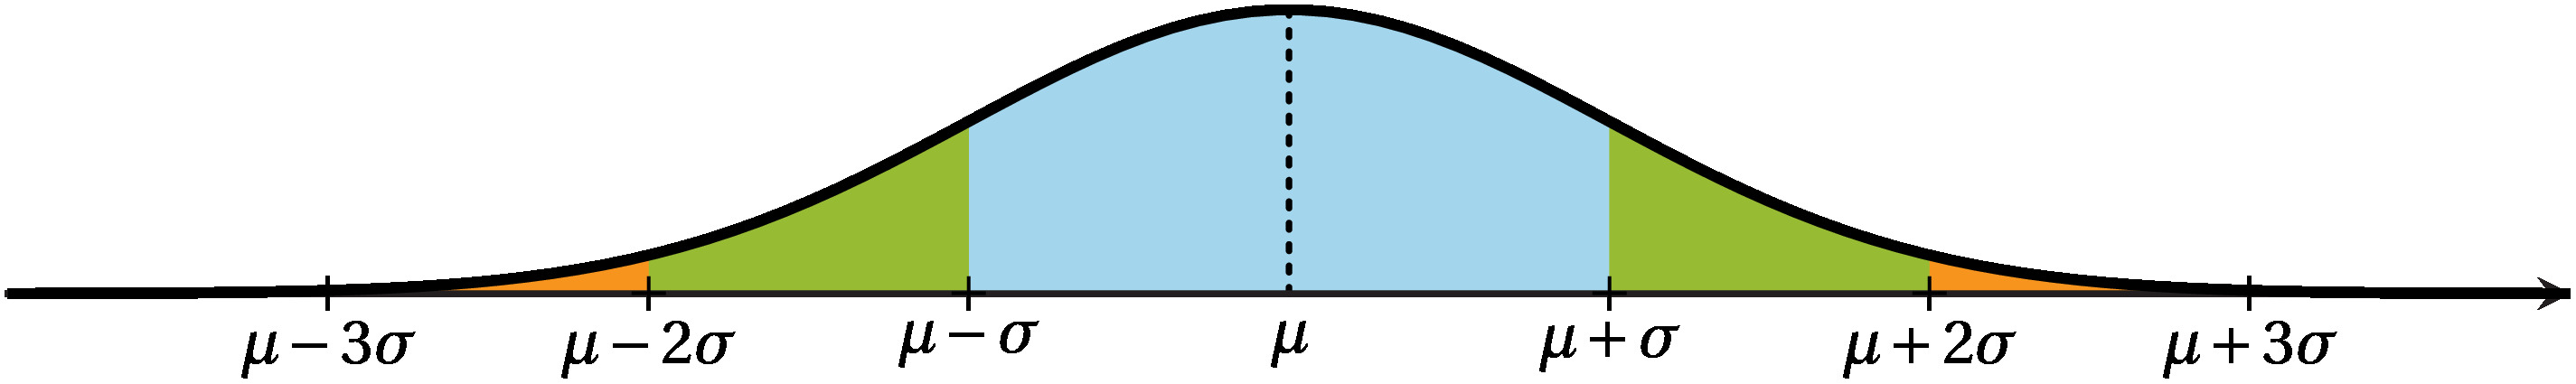
\includegraphics{./TS-Variables-15}




où l'aire du domaine en bleu est environ 0,68, l'aire du domaine en bleu et vert est environ 0,954 et l'aire du domaine en bleu, vert et orange (jusqu'à $\mu-3\sigma$ et $\mu+3\sigma$) est environ 0,997.
\end{propriete}




~~

\end{document}